\documentclass[10pt,twocolumn,letterpaper]{article}

\usepackage{cvpr}
\usepackage{times}
\usepackage{epsfig}
\usepackage{graphicx}
\usepackage{amsmath}
\usepackage{amssymb}
\usepackage{float}
\usepackage{algorithm}
\usepackage{algpseudocode}
\usepackage{biblatex}
\usepackage{booktabs}
\bibliography{/home/shi/Documents/UFMG/CN/TP2/doc/egbib.bib}
\graphicspath{{/home/shi/Documents/UFMG/CN/TP2/doc/images}}

% Include other packages here, before hyperref.

% If you comment hyperref and then uncomment it, you should delete
% egpaper.aux before re-running latex.  (Or just hit 'q' on the first latex
% run, let it finish, and you should be clear).
\usepackage[breaklinks=true,bookmarks=false]{hyperref}
\graphicspath{{./images/}}

\cvprfinalcopy % *** Uncomment this line for the final submission

\def\cvprPaperID{****} % *** Enter the CVPR Paper ID here
\def\httilde{\mbox{\tt\raisebox{-.5ex}{\symbol{126}}}}

% Pages are numbered in submission mode, and unnumbered in camera-ready
%\ifcvprfinal\pagestyle{empty}\fi
\begin{document}

%%%%%%%%% TITLE
\title{Trabalho Prático II - ACO}

\author{Daniel Carneiro\\
Universidade Federal de Minas Gerais\\
Belo Horizonte, MG, 31.270-901\\
{\tt\small dennys@ufmg.br
% For a paper whose authors are all at the same institution,
% omit the following lines up until the closing ``}''.
% Additional authors and addresses can be added with ``\and'',
% just like the second author.
% To save space, use either the email address or home page, not both
}
}

\maketitle
%\thispagestyle{empty}

%%%%%%%%% ABSTRACT
\begin{abstract}
   O objetivo desse trabalho foi a implementação de um algoritmo de \textbf{Ant Colony Optimization} (ACO) para o \textbf{longest path problem}. O algoritmo foi implementado em python $3.10$ e utiliza a biblioteca externa numpy.
\end{abstract}

%%%%%%%%% BODY TEXT
\section{Introduction}

\textbf{Ant Colony Optimization} (ACO) é uma metaheurística utilizada para resolver problemas que podem ser reduzidos a encontrar bons caminhos em grafos. Nessa metaheurística utilizamos formigas artificiais para caminhar no gráfico e, imitando o comportamento de formigas reais, deixar feromônios no melhor caminho para guiar (probabilisticamente) as outras formigas para caminhos bons.

Nesse trabalho foi estudado e implementado um algoritmo de ACO com o objetivo de aproximar uma solução para o \textbf{longest path problem}, no qual o objetivo é encontrar o maior caminho em um grafo entre quaisquer dois vértices. Nas próximas sessões iremos descrever as decisões de implementação, otimização de parâmetros, experimentos e resultados.

\section{Decisões de Implementação}

A versão de ACO implementada foi a $\mathcal{MMAS}$ (Max Min Ant System) \ref{alg:aco}, utilizando o descrito no livro \citetitle{Dorigo2004} (\Citeauthor{Dorigo2004})\cite{Dorigo2004}. As decisões tomadas foram descritas a seguir.

\begin{algorithm}
   \caption{ACO}\label{alg:aco}
   \begin{algorithmic}
      \State $t \gets 1$
      \State best $\gets$ (0, [])
      \State Initialize graph with $t_{max}$ pheromones on every edge
      \While{$t < \text{maxIt}$}
      \State Build popSize solutions in parallel $\to S$
      \State itbest $\gets (\max{S}.\text{length}, \max{S}.\text{path})$
      \If{itbest[0] $>$ best[0]}
      \State best $\gets$ itbest
      \EndIf
      \State $r \gets $ Choose from \{best, itbest\} with probabilities ($t/$maxIt, $1-t/$maxIt)
      \State Update pheromones with $r.$path
      \State $t \gets t + 1$
      \EndWhile
      \State \Return best
   \end{algorithmic}
\end{algorithm}

\subsection{Paralelismo}

O algoritmo \ref{alg:aco} mostra como que o paralelismo foi implementado, nós construímos os caminhos em paralelo, e atualizamos os feromônios de maneira sequencial.

\subsection{Representação da Solução}

A solução é representada pela sequência de vértices que visitamos (e.g. $v_2v_1v_3$).

\subsection{Probabilidade de Transição}

A probabilidade de transição por uma aresta é dada pela equação

$$
   \frac{w^\alpha n^\beta}{\sum_{v_i \in N} w_i^\alpha n_i^\beta}
$$

Onde $w$ é o feromônio da aresta, $n$ é o peso, $N$ é a vizinhança, e $n_i$ e $w_i$ são o peso e o feromônio da aresta que conecta o vértice atual a $i$.

\subsection{Atualização dos Feromônios}

O $\mathcal{MMAS}$ têm como característica a utilização de um limite mínimo e máximo para os feromônios, nesse trabalho foi utilizado um limite variável onde $t_{max}$ é o tamanho do caminho sendo utilizado para atualizar os feromônios dividido pela taxa de evaporação e $t_{min}$ é $t_{max}\cdot((1-\sqrt[n]{0.05})/((avg-1)\sqrt[n]{0.05}))$ onde $n$ é o número de vértices do grafo e $avg$ é a média de arestas que saem de um vértice.

Como explicitado no algoritmo \ref{alg:aco}, no inicio das iterações nós atualizamos o feromônio utilizando com maior probabilidade o melhor caminho encontrado naquela iteração para promover exploração, e depois se torna mais provável que utilizemos o melhor caminho encontrado até então para promover o exploitation.

\subsection{Parâmetros}

Os parâmetros ajustáveis pelo usuário são o número de iterações, o número de formigas, $\alpha$, $\beta$ e a taxa de evaporação $\rho$. Esses parâmetros foram ajustados para o problema de caminho mais longo na sessão a seguir.

\section{Otimização de Parâmetros}

Os parâmetros iniciais utilizados foram os da tabela \ref{tab:paraminit} como sugerido por \citeauthor{Dorigo2004}\cite{Dorigo2004}. Todos os parâmetros foram ajustados utilizando o arquivo de testes \textit{entrada3.txt}, por possuir o maior número de caminhos possíveis e, portanto, maior variedade de soluções.

Em todos os testes foram realizadas $30$ execuções, e todos os dados representados nos gráficos são a média dos resultados obtidos nas $30$ execuções.

\begin{table}[H]
   \caption{Parâmetros iniciais, $\rho$ é a taxa de evaporação, $C^{fn}$ é o custo da solução obtida pela heurística gulosa de vizinho mais distante.}
   \centering
   \begin{tabular}{|c|c|}
      \hline
      Parâmetro           & Valor           \\
      \hline\hline
      Feromônio Inicial   & $1/\rho C^{fn}$ \\
      \hline
      Número de Formigas  & $10$            \\
      \hline
      $\beta$             & $5$             \\
      \hline
      $\rho$              & $0.02$          \\
      \hline
      $\alpha$            & $1$             \\
      \hline
      Número de iterações & $400$           \\
      \hline
   \end{tabular}
   \label{tab:paraminit}

\end{table}

\subsection{Número de Formigas}

Os gráficos \ref{fig:popbest} e \ref{fig:poptime} mostram o impacto do número de formigas na melhor solução e no tempo de execução. Foi determinado que os ganhos pelo aumento de população não justificam o aumento de tempo de execução. Por isso o número de formigas foi mantido em $10$.

\begin{figure}[H]
   \begin{center}
      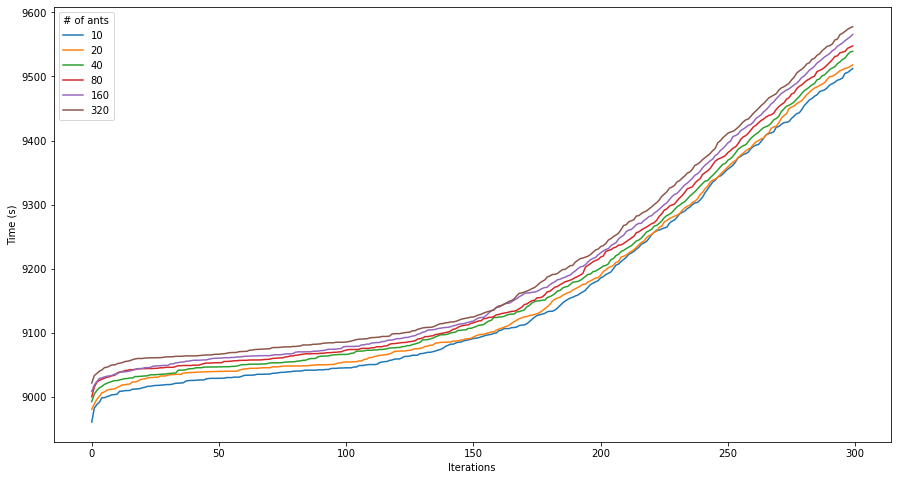
\includegraphics[width=\linewidth]{popbest}
   \end{center}
   \caption{Melhor solução encontrada para diversos números de formigas}
   \label{fig:popbest}
\end{figure}

\begin{figure}[H]
   \begin{center}
      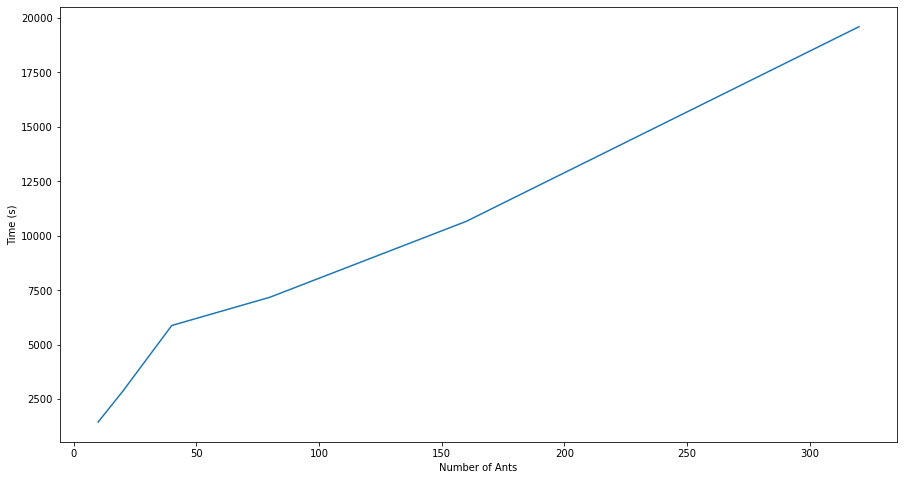
\includegraphics[width=\linewidth]{poptime}
   \end{center}
   \caption{Tempo de execução por número de formigas}
   \label{fig:poptime}
\end{figure}


\subsection{Iterações}

O gráfico \ref{fig:itsbest} mostra a melhor solução encontrada por iteração, e o gráfico \ref{fig:ittime} mostra o tempo de execução do teste para números máximos de iterações diferentes. Como o algoritmo é $O(n)$ em relação ao número de iterações e há ganhos até $700$ iterações, foi escolhido $700$ para o número de iterações.

\begin{figure}[H]
   \begin{center}
      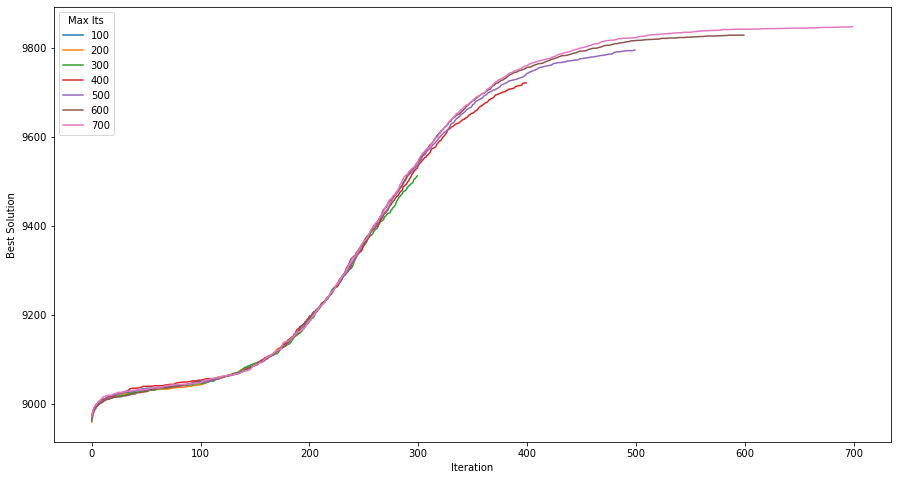
\includegraphics[width=\linewidth]{its}
   \end{center}
   \caption{Melhor solução encontrada por iteração}
   \label{fig:itsbest}
\end{figure}

\begin{figure}[H]
   \begin{center}
      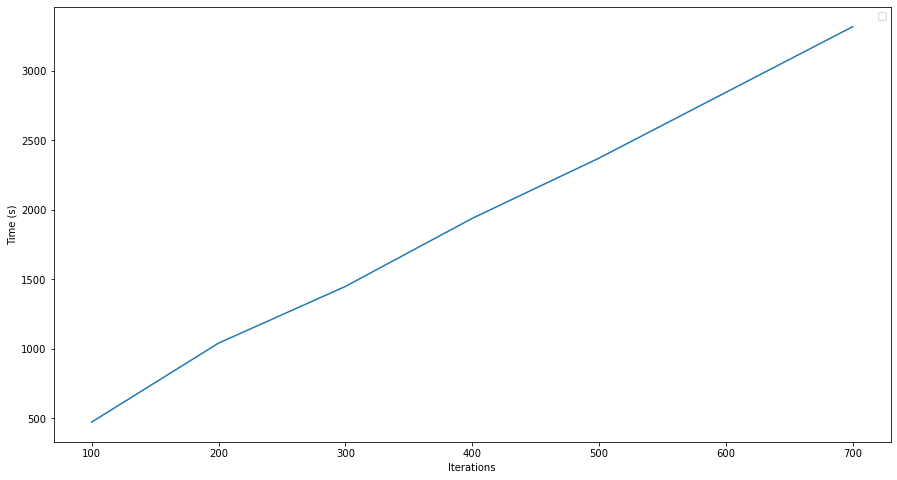
\includegraphics[width=\linewidth]{ittime}
   \end{center}
   \caption{Tempo de execução por iteração}
   \label{fig:ittime}
\end{figure}



\subsection{Beta}

O gráfico \ref{fig:beta} mostra o valor da melhor solução encontrada para diferentes valores de $\beta$. O $\beta$ basicamente é o peso que damos para seguir a aresta de maior comprimento, e como quanto maior o $\beta$ melhor a solução, surge uma dúvida se na verdade a heurística de vizinhos mais distantes é melhor que o ACO implementado. Para testar essa hipótese foi encontrada a melhor solução para essa heurística setando $\alpha$ em $0$ e iniciando uma formiga em cada vértice do grafo. Ficou claro que os feromônios ainda tinham um papel importante, e a implementação do ACO foi justificada. Foi escolhido $\beta = 75$.

\begin{figure}[H]
   \begin{center}
      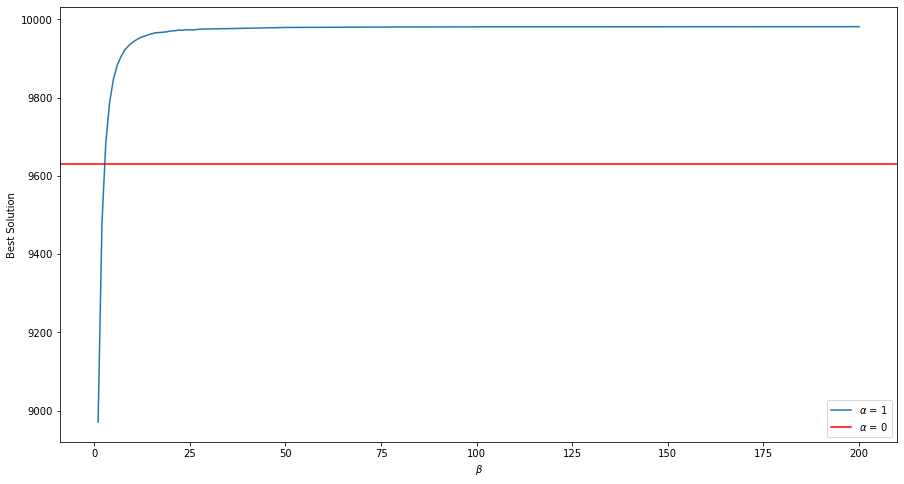
\includegraphics[width=\linewidth]{beta}
   \end{center}
   \caption{Melhor solução encontrada para diferentes valores de $\beta$}
   \label{fig:beta}
\end{figure}

\subsection{Rho}

O gráfico \ref{fig:rho} mostra o valor da melhor solução para diferentes valores de $\rho$, como $0.08$ obteve os melhores resultados e uma convergência mais suave, optou-se por utilizar $\rho = 0.08$.

\begin{figure}[H]
   \begin{center}
      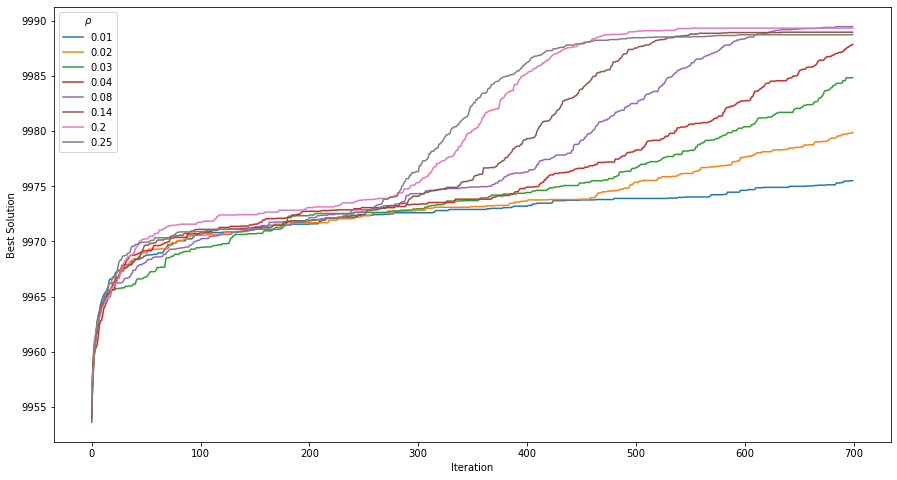
\includegraphics[width=\linewidth]{rho}
   \end{center}
   \caption{Melhor solução encontrada para diferentes valores de $\rho$}
   \label{fig:rho}
\end{figure}

\subsection{Alpha}

Talvez não faça tanto sentido ajustar $\alpha$, uma vez que o ajuste de $\beta$ já seja um ajuste indireto de $\alpha$, porém com objetivo explorativo, também realizamos um experimento para $\alpha$. Os resultados estão ilustrados pelo gráfico \ref{fig:alpha}. Foi observado que $\alpha=2$ obteve resultados marginalmente melhores que $\alpha=1$ consistentemente em múltiplas execuções do teste. Isso provavelmente ocorreu pois o ajuste de $\rho$ alterou o impacto que os feromônios têm para encontrar um melhor caminho. Optou-se então por utilizar $\alpha=2$.

\begin{figure}[H]
   \begin{center}
      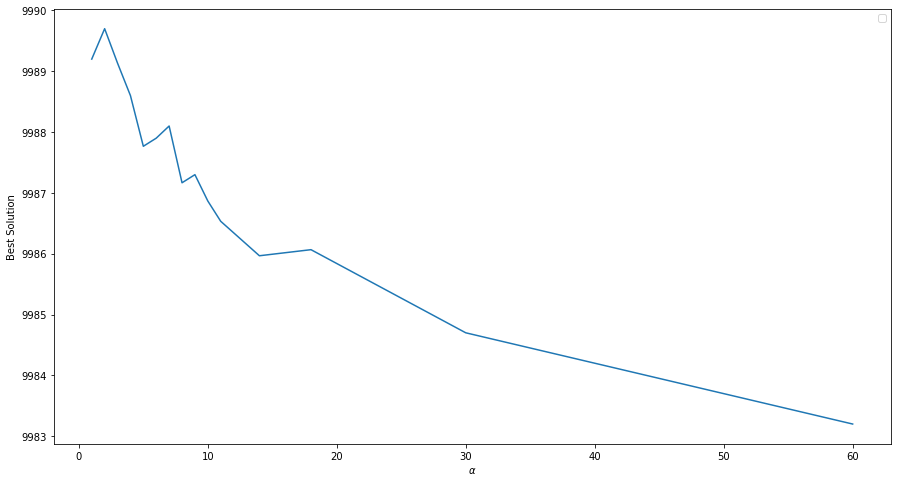
\includegraphics[width=\linewidth]{alpha}
   \end{center}
   \caption{Melhor solução encontrada para diferentes valores de $\alpha$}
   \label{fig:alpha}
\end{figure}

\subsection{Parâmetros Finais}

A tabela \ref{tab:param} apresenta os parâmetros escolhidos. E o gráfico \ref{fig:final} apresenta o resultado da execução com esses parâmetros.

\begin{table}[H]
   \caption{Parâmetros finais}
   \centering
   \begin{tabular}{|c|c|}
      \hline
      Parâmetro          & Valor  \\
      \hline\hline
      Iterações          & $700$  \\
      \hline
      Número de Formigas & $10$   \\
      \hline
      Beta               & $75$   \\
      \hline
      Rho                & $0.08$ \\
      \hline
      Alpha              & $2$    \\
      \hline
   \end{tabular}
   \label{tab:param}

\end{table}

\begin{figure}[H]
   \begin{center}
      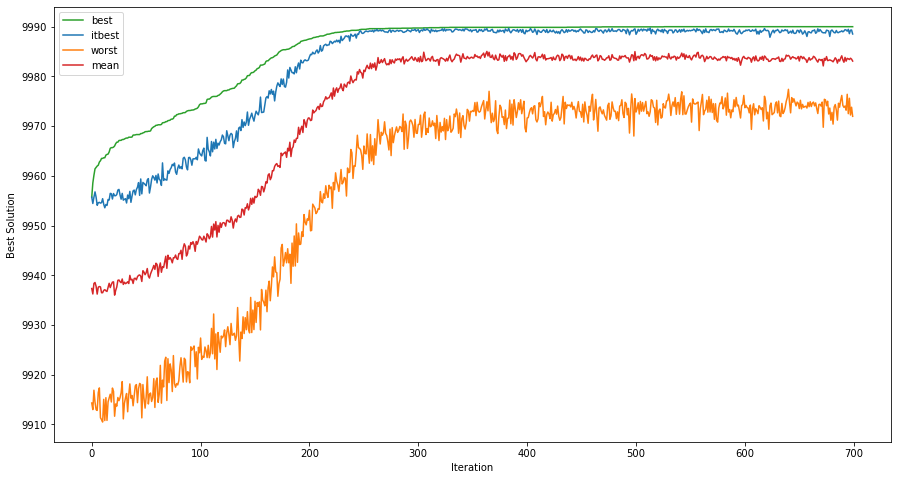
\includegraphics[width=\linewidth]{final}
   \end{center}
   \caption{Melhor solução até então (best-so-far), melhor solução da iteração atual, pior solução e solução média para os parâmetros finais.}
   \label{fig:final}
\end{figure}


Na sessão seguinte iremos descrever os resultados do algoritmo para os três conjuntos de dados.

\section{Resultados}

Nessa sessão iremos apresentar três tabelas (\ref{tab:1}, \ref{tab:2}, \ref{tab:3}) com estatísticas descritivas sobre as soluções encontradas.

\begin{table}[H]
   \caption{Resultados para \textit{entrada1.txt}}
   \label{tab:1}
   \begin{tabular}{lrrrrrrrr}
      \toprule
      count & mean  & std \\
      \midrule
      30  & 990 & 0 \\
      \bottomrule
   \end{tabular}
\end{table}

\begin{table}[H]
   \caption{Resultados para \textit{entrada2.txt}}
   \label{tab:2}
   \begin{tabular}{lrrrrrrrr}
      \toprule
      count & mean       & std      & min   & 25\% &max   \\
      \midrule
      30  & 175.56667 & 0.93526 & 173 & 176 & 176 \\
      \bottomrule
   \end{tabular}

   \begin{table}[H]
   \end{table}
   \caption{Resultados para \textit{entrada3.txt}}\label{tab:3}

   \begin{tabular}{lrrrrrrrr}
      \toprule
      count & mean   & std \\
      \midrule
      30  & 9990 & 0 \\
      \bottomrule
   \end{tabular}

\end{table}


\section{Conclusão}

O fato do desvio padrão para as entradas $1$ e $3$ serem $0$ é um indicio de que possivelmente o algoritmo encontrou o ótimo toda vez. Para a entrada $2$ temos que no percentil $.25$ encontramos o ótimo. Isso também indica que para os parâmetros finais o número de formigas e o número de iterações são maiores do que o necessário, isso é evidenciado ainda mais pelo gráfico \ref{fig:final} que na iteração $300$ o algoritmo já havia convergido. Portanto poderíamos executar o algoritmo mais rapidamente sem comprometer qualidade da solução, por exemplo definindo uma condição de parada após $x$ execuções sem melhora, ou simplesmente diminuindo o número máximo de execuções diretamente.

Seria interessante futuramente revisitar a etapa de otimização de parâmetros partindo dos parâmetros atuais, para otimizar o tempo de execução e qualidade das soluções. Seria interessante também alterar a ordem de otimização de parâmetros, por exemplo otimizando $\rho$ antes de $\beta$.

\printbibliography
\end{document}
